%\documentclass{article}
%\usepackage{graphicx,subfigure}
%\begin{document}

\begin{figure}[!h]
  \centering
   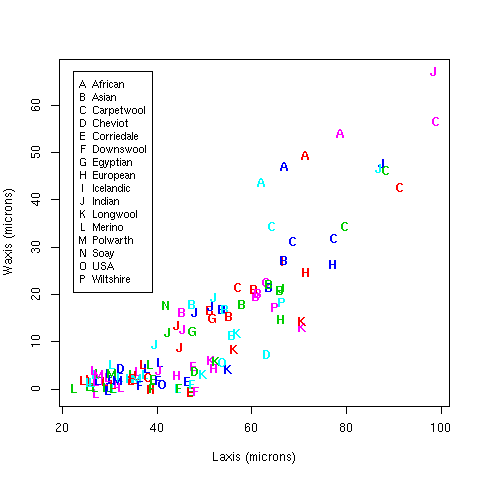
\includegraphics[width=1.0\textwidth]{LWalltype.png}
  \caption{Plot of breed means of secondary fibre diameter (Ds) and primary fibre diameter (Dp) for 126 flocks sampled by Carter(1968)~\cite{cart:68}. The axes have been rotated 45 degrees so that L-axis represents projections onto the line $D_{p}/D_{s} = 1$, and W-axis represents projections onto a line at right angles to the L-axis. The W-axis is interpreted a two-coatedness, and the L-axis is interpreted a large fibres. The breeds have been grouped into a {\em breed type} which in some cases is an individual breed and in other cases is a country of origin. }
  \label{fig:LWalltype}
\end{figure}

%\end{document}

